\RequirePackage[]{lineno}
\documentclass[12pt]{article}
\usepackage{caption}
\usepackage{times}
\usepackage{setspace}
\usepackage{longtable}
\usepackage{amsmath}
\usepackage{booktabs}
\usepackage{float}
\usepackage{mathpazo}
\usepackage{times}
\usepackage{tikz}
\usepackage{graphicx}
\usepackage[hmargin=2.25cm, vmargin=2cm, headheight=15.5pt]{geometry}
\usepackage{multirow}
\usepackage{tcolorbox}
\usepackage{multicol}
\usepackage{tabularx}
\usepackage{rotating}
\usepackage{pdflscape}
\captionsetup[figure]{font=small}
\captionsetup[table]{font=small}

\usetikzlibrary{arrows,calc}
\geometry{margin=1in}

%\captionsetup{font=doublespacing, size= footnotesize}% Double-spaced float captions
\doublespacing
\DeclareCaptionJustification{double}{\DoubleSpacing}
% Reasonable page setup


\usepackage[]{natbib}
\bibpunct[; ]{(}{)}{;}{a}{,}{;}

% to avoid things being lost to overleaf comment bubbles
\long\def\authornote#1{%
    \leavevmode\unskip\raisebox{-3.5pt}{\rlap{$\scriptstyle\dagger$}}%
    \marginpar{\raggedright\hbadness=10000
        \def\baselinestretch{0.8}\tiny
        \it #1\par}}
\newcommand{\DBS}[1]{\authornote{DBS: #1}}
\newcommand{\ACL}[1]{\authornote{ACL: #1}}

\usepackage{authblk}
\renewcommand\Affilfont{\small}

\newenvironment{abox}[1]{
  \begin{tcolorbox}[float,title=#1, colback=blue!4]
  \fontsize{9}{10}\selectfont
  \begin{multicols}{2}
}{
  \end{multicols}
  \end{tcolorbox}
}


\newenvironment{ecolettcover}{\maketitle}{\clearpage}
\newenvironment{ecolettabstract}{\clearpage\section*{Abstract}}{\clearpage}
\tikzset{
	%Define standard arrow tip
	>=stealth',
	%Define style for different line styles
	help lines/.style={dashed, thick},
	axis/.style={<->},
	important line/.style={thick},
	connection/.style={thick, dotted},
}

%\title{The structural sensitivity of competition models: how model formulation changes our predictions of species coexistence}
\title{Coexistence of alleles: insights of Modern Coexistence Theory into the maintenance of genetic diversity}
\author[1]{Alba Cervantes-Loreto}
\author[1]{Michelle L.\ Maraffini}
\author[1]{Daniel B.\ Stouffer}
\author[1]{Sarah P.\ Flanagan}


\affil[1]{Centre for Integrative Ecology, School of Biological Sciences\\ University of Canterbury, Christchurch 8140, New Zealand}



% Include the date command, but leave its argument blank.
\date{}

%%%%%%%%%%%%%%%%% END OF PREAMBLE %%%%%%%%%%%%%%%%
\let\oldequation\equation
\let\oldendequation\endequation

\renewenvironment{equation}
  {\linenomathNonumbers\oldequation}
  {\oldendequation\endlinenomath}

% \pagestyle{empty}

\begin{document}
\linenumbers
% Double-space the manuscript.
\baselineskip30pt
\maketitle

\begin{ecolettcover}

%\centerline{{\sc Running Title:} The structural sensitivity of competition models}
\begin{center}
\begin{tabular}{ll}
\hline \\

\bf{Words in abstract}         & to be determined \\
\bf{Words in manuscript}       & to be determined\\
\bf{Number of references}      & to be determined  \\
\bf{Number of figures}			& to be determined \\
\bf{Number of tables} 			& 2 \\
\bf{Number of text boxes}		& 0 \\
\bf{Corresponding author}      & Alba Cervantes-Loreto \\
\bf{Phone}                     & +64~369~2880 \\

\bf{Email}                     & alba.cervantesloreto@pg.canterbury.ac.nz \\
                                                                        \\
\hline
\end{tabular}
\end{center}

\maketitle

\end{ecolettcover}
%%%%%%%%%%%%%%%%%%%
\section{Introduction}
The question of how genetic variation is maintained, despite the effects of selection and drift, continues to be central to the study of evolutionary biology \citep{walsh_evolution_2018}. Classical explanations include overdominance (heterozygote advantage) or frequency-dependent selection, but in the modern era of genomic data, all patterns of variation that exceed the expected variation under neutrality tend to be categorized broadly as balancing selection, regardless of the evolutionary mechanism \citep{mitchell-olds_which_2007}.  One of the evolutionary mechanisms coined under balancing selection is sexually antagonistic selection, which occurs when the direction of natural selection on traits or loci differs between the sexes \citep{connallon2018environmental}.

Sexually antagonistic selection has been identified as a powerful engine of speciation that in some cases can mantain polymorphisms of otherwise dis-advantageous alleles in a population \citep{gavrilets2014sexual}. The effect of sexually antagonistic selection, however, has been generally studied under strong simplifying assumptions such as constant population sizes and homogeneous environments (e.g.,\citet{kidwell1977regions, pamilo1979genic, immler2012ploidally}). Few studies have explored the effect of sexually antagonistic selection on the maintenance of polymorphism with more realistic assumptions. Excepctions include \citet{connallon_evolutionary_2018} who found that classical predictions break down when fluctuations in the environment combined with life-history traits allow local adaptations and promote the maintenance of genetic diversity. The effect of environmental fluctuations without local adaptation, however, has not been studied in the context of sexually antagonistic selection to the best of our knowledge.


The contribution of environmental fluctuations to genetic variability remains a debated issue in evolutionary biology. Classic theoretical models predict that temporal fluctuations in environmental conditions are unlikely to maintain a genetic polymorphism \citep{hedrick1974genetic,hedrick1986genetic}. However, other studies have found that fluctuating selection can maintain genetic variance on sex--linked traits \citep{reinhold2000maintenance}, or in populations where generations overlap \citep{ellner1994role, ellner1996patterns}. Similarly, temporal changes in population sizes have been shown to mitigate the effect of genetic drift in small populations \citep{pemberton1996maintenance}, and in annual plant systems \citep{nunney2002effective}. Thus, both fluctuations in selection and population sizes could dramatically change the effect of sexually antagonistic selection in the maintenance of genetic diversity.


Importantly, progress requires more than just identifying if fluctuations can maintain genetic diversity in a population, but to quantify how exactly they contribute to its maintenance \citep{ellner2016quantify}. Modern coexistence theory (MCT) provides a powerful conceptual framework to do so \citep{Chesson2000,chesson1994multispecies, barabas_chessons_2018}. Although its core ideas were formalized in an ecological context \citep{chesson1994multispecies,chesson2000general}, this framework provides the necessary tools to examine the relative contributions of fluctuations to diversity maintenance, which can also be applied to evolutionary contexts  \citep{ellner1996patterns,reinhold2000maintenance}. From an ecological perspective, polymorphism of sexually antagonistic alleles is equivalent to the coexistence of species, and the fixation of either one of the alleles in a population is equivalent to competitive exclusion. The coexistence of alleles, thus, can be examined through the same lens as the coexistence of competing species.

Here, we seek to explicitly apply recent  advances in MCT to the question of how
polymorphism is maintained under sexually antagonistic selection.  We examined how fluctuations in selection values, fluctuations in population sizes, and their interactions can stabilize or hinder the coexistence of alleles. In particular, we examined  i) Can fluctuations in population sizes and selection values allow sexually antagonistic alleles to coexist when differences in their fitness would typically not allow them to? and ii) What is the relative contribution of different types of fluctuations that allow two sexually antagonistic alleles to be maintained in a population? Our study provides the tools to analyze evolutionary dynamics from a novel perspective and contributes to answering long-lasting questions regarding the effect of non-constant environments on genetic diversity.



\section{Methods}

We first present  a model that describes the evolutionary dynamics of sexually antagonistic alleles and show how changes in allele frequencies can be expressed in terms of growth rates, a necessary condition for analyses done using MCT. We continue by simulating different scenarios of alleles invading a population, where we allowed population sizes, selection values, both, or neither to vary. Finally, we examine the results of our simulations through a MCT lens by calculating the contribution of each of these fluctuations in the coexistence of alleles across the parameter space of sexually antagonistic selection.


\subsection*{Population dynamics of sexually antagonistic alleles}

 As most population genetic models of sex-dependent selection, our model considered evolution at single, biallelic  locus with frequency and density independent effects on the relative fitness of females and males \citep{wright1942statistical,kidwell1977regions, immler2012ploidally}\ACL{Add more recent refs, sarahs suggestions and e.g.,}. We examined the dynammics of two  sexually antagonistic alleles, $j$ and $k$, that affect fitness in the haploid state. We assumed allele $j$ always has a high fitness in females ($w_{jf} = 1$), but variable fitness in males ($w_{jm} < 1$); and allele $k$ has a high fitness in males ($w_{km} = 1$), but variable fitness in females ($w_{kf} < 1 $). The selection against allele $j$ in males is therefore $S_{m}= 1 - w_{jm}$, and the selection against allele $k$ in females is $S_{f}= 1 - w_{kf}$.

 The frequency of each allele in each sex at the beginning of a life-cycle at time $t$ is given by:
 \begin{equation}
     p_{jm,t}= \frac{n_{jm,t}}{N_{m,t}}
     \label{first_pop}
 \end{equation}
 \begin{equation}
     p_{jf,t}= \frac{n_{jf,t}}{N_{f,t}}
 \end{equation}
 \begin{equation}
     p_{km,t}= \frac{N_{m,t}-n_{jm,t}}{N_{m,t}}
 \end{equation}
 \begin{equation}
     p_{kf,t}= \frac{N_{f,t}-n_{jf,t}}{N_{f,t}}
 \end{equation}
 where $N_{m,t}$ and $N_{t,t}$ are the numbers of males and females in a population at time $t$, $n_{jf,t}$ is the number of females $f$ with allele $j$, and $n_{jm,t}$ is the number of males $m$ with allele $j$ at time $t$, respectively.

 The individuals in the population mate at random before selection occurs, and therefore the frequency of offspring with allele $j$ after mating, $p'_{j,t}$ can be expressed as:
 \begin{equation}
    p'_{j,t}= \frac{(N_{m,t}n_{jf,t}+ N_{f,t}n_{jm,t})}{2 N_{f}N_{m}} \,.
    \label{pprime}
 \end{equation}
 Selection acts upon these offspring in order to determine the allelic frequencies in females and males in the next generation, $t+1$. As an example the frequency  of females with allele $j$ after selection is given by:
 \begin{equation}
    p^{\prime}_{jf, t+1}= \frac{n_{jf, t+1}}{N'_{f,t+1}} = \frac{p'_{j}w_{jf}}{p'_{j}w_{jf}+ (1-p'_{j})w_{kf}}
    \label{next_gen}
 \end{equation}

 The logarithmic growth rate of $j$ in females, is therefore given by the number of females with allele $j$ after selection, divided by the original number of females carrying allele $j$:



 \begin{equation}
     r_{jf,t} = \ln \left( \frac{n'_{jf, t+1}}{n_{jf,t}} \right)
     \label{canonical}
 \end{equation}

 An equivalent expression for the per capita growth rate of allele $j$ in males $m$ can be obtained by exchanging $f$ for $m$ across the various subscripts in this expression.

 Allelic coexistence in a sexual population, however, is ultimately influenced by growth and establishment of an allele across both sexes. Therefore, the full growth rate of allele $j$ across the entire population of females \emph{and} males is given by:
 \begin{equation}
     r_{j} = \ln \left( \frac{n'_{jf, t+1} + n'_{jm, t+1} }{n_{jf,t} + n_{jf,t} }  \right) \,.
     \label{full}
 \end{equation}

An equivalent expression describes $r_{k}$, the growth rate of allele $k$.

Selection mantains both alleles in the population under the condition that:

\begin{equation}
\frac{S_{m}}{1+S_{m}} < S_{f} < \frac{S_{m}}{1-S_{m}}
\label{selection}
\end{equation}
Thus,the maintenance of polymorphism of sexually antagonistic alleles is solely determined by the values of $S_{m}$ and $S_{f}$. Note that in our model, the values $S_{m}$ and $S_{f}$ can take are bounded from $0$ to $1$. Therefore the parameter space of sexually antagonistic selection is within the range $ 0< S_{m}, S_{f} < 1$. Classic theoretical models predict that in constant environments, only in $\approx 0.38$ of the selection parameter space alleles can coexist \citep{kidwell1977regions,pamilo1979genic,connallon_evolutionary_2018}.  If fluctuations in population sizes or selection values have an effect on the coexistence of sexually antagonistic alleles, it would be reflected in increases or decreases of the proportion of the parameter space of selection where polymorphism is maintained.



\subsection*{Simulations}

%Although the evolutionary dynamics of sexually antagonistic selection is often explored through changes in alleles' frequencies, MCT requires population dynamics to be expressed as growth rates of the competing alleles, as we show in Eqn.\ref{full}.
Typically, MCT would require decomposing alleles' growth rates (e.g., Eqn.~\ref{full}) analytically to examine the relative contributions of different types of fluctuations to their coexistence \citep{barabas_chessons_2018}. Although we present an analytical approach in the Supporting Information, our general solution is not easily interpretable and soon becomes mathematically intractable (S1 Supporting Information). Thus, we opted for an extension of MCT that provides the flexibility to examine the contributions of different processes to coexistence using simulations \citep{ellner_expanded_2019, shoemaker2020}.

%Our approach first consisted, following \citep{shoemaker2020}, of incorporating fluctuations in selection and population sizes into our population dynamics model. Then, we performed simulations of each allele invading a population that experiences the aforementioned fluctuations. Finally, we looked at the relative contributions of each type of fluctuation that allowed each allele to establish in a population.


For each simulation, we examined coexistence outcomes across the selection parameter space of sexually antagonistic selection ($0 < S_{m}, S_{f} < 1$). To do so, we partitioned the parameter space into a grid of $50 \times 50$, which yielded 2500 pairwise combinations of different $w_{jm}$ and $w_{kf}$ values. For each pairwise combination of $w_{jm}$ and $w_{kf}$, as we detail in the next sections, we iterated our model while controlling the effect size of  fluctuations in fitness values ($\sigma_{w}$), fluctuations in population sizes ($\sigma_{g}$) and their correlations ($\rho_{w}$ and $\rho_{g}$ respectively). Then, we performed simulations of each allele invading a population, determined coexistence outcomes, and the relative contribution of each type of fluctuation. Finally, we calculated for each simulation, the proportion of the parameter space that allowed alleles to coexist.

We explored all of  the combinations of low , intermediate  and high fluctuations  in fitness values and population sizes, with different extents of correlations between fluctuations (Table \ref{tab:fluctuations}).  As a control simulation, we set $\sigma_{w}= 0.001$ and  $\sigma_{g}=0.001$, with no correlation between fluctuations. For each one of the factorial combinations of $\sigma_{g}$, $\sigma_{w}$, $\rho_{g}$ and $\rho_{w}$ (Table \ref{tab:fluctuations}), we performed invasion simulations across the parameter space of selection. We ran ten replicates per parameter combination, which resulted in 3780 simulations.

\subsubsection*{Timeseries}


To incorporate the effects of fluctuations into our population dynamics model we generated independent timeseries of fluctuations in fitness values and population sizes. In the case of fluctuations in selection values, for a given value of $w_{jm}$ and $w_{kf}$ (i.e., a fixed point in the selection parameter space), we generated a timeseries of 500 timesteps made up of correlated fluctuations of $w_{jm}$ and $w_{kf}$. We controlled the effect size of  fluctuations in fitness values ($\sigma_{w}$) and its correlation ($\rho_{w}$) by  using the Cholesky factorization of the variance-covariance matrix:

\begin{equation}
C_{w} = \begin{bmatrix}
\sigma_{w}^{2} & \rho_{w} \sigma_{w}^{2} \\
\rho_{w} \sigma_{w}^{2} & \sigma_{w}^{2}
\end{bmatrix}
\label{covmat}
\end{equation}

We multiplyed Eqn.~\ref{covmat} by a ($2 \times 500$) matrix of random numbers from a normal distribution with mean 0 and unit variance, which yielded $\gamma_{j}$ and $\gamma_{k}$. Then, we calculated the value of $w_{jm}$ at time $t+1$ as $w_{jm,t+1} = w_{jm}^{\gamma_{j,t}}$. We calculated the value of $w_{kf,t+1}$  analogously.

Similarly, we generated a timeseries of 500 timesteps made up of correlated fluctuations in population sizes. We chose values of $N_{m}$ and $N_{f}$ of 200 individuals each as the initial value of population sizes throughout our simulations. We performed a Cholesky factorization of the variance-covariance matrix, controlling the effect size of fluctuations in population sizes with $\sigma_{g}$ and their correlation with $\rho_{g}$. Similar to our previous approach, we multiplied this factorization by a random matrix of uncorrelated random variables, which yielded $\gamma_{m}$ and $\gamma_{f}$. Finally, we calculated the number of males in the population at time $t+1$ as $N_{m,t+1} = N_{m} + \gamma_{m,t}$. We calculated the value of $N_{f,t+1}$  analogously. We bounded the values population sizes could take so there were no negative population sizes, since that would not be biologically plausible. We did not impose an upper bound to the values population sizes could take. \ACL{We did not impose any bounds to sex ration, nor total population sizes, I don't know if that is worth mentioning}

Finally, we performed simulations where our population dynamics model (Eqns.~\ref{first_pop} to \ref{full}) iterated over 500 timesteps while allowing selection values and population sizes to fluctuate in each timestep. We started each simulation with the initial values of $N_{m}$ and $N_{f}$ described before and equal frequencies of allele $j$ and allele $k$ in each sex. For each timestep $t$ in our simulations, the values of $w_{jm}$ $w_{kf}$, $N_{m}$ and $N_{f}$ used to calculate allele´s frequencies in in timestep $t$ (e.g., Eqn.~\ref{next_gen}), corresponded to the $t$ values calculated in each timeseries, as described previously. This approach yielded a final timeseries that captured the dynamics of sexually antagonistic alleles, with fluctuating values of selection and population sizes.

\vspace{5mm}
\noindent\textbf{Invasion simulations}

 Modern coexistence theory has shown that coexistence is promoted by mechanisms that give species a population growth rate advantage over other species when they become rare \citep{chesson_stabilizing_1982, chesson2003quantifying, barabas_chessons_2018}. Typically, one species is held at its \textit{resident} state, as given by its steady-state abundances while the rare species is called the \textit{invader}. In the context of alleles in a population, an allele is an \textit{invader} when a mutation occurs that introduces that allele into a population in which it is absent (e.g., if in a population with only $k$ alleles, a random mutation made one individual carry the $j$ allele). Within sexually antagonistic selection, each allele has two pathways of invasion, depending on whether the mutation arises in a female or in a male. If an alleles' \textit{invasion growth rate} (or the average instantaneous population growth rate when rare) is positive, it buffers it against extinction, maintaining its persistence in the population.  Coexistence, and hence polymorphism, occurs when both alleles have positive invasion growth rates.

To study the dynamics of sexually antagonistic alleles through this framework, we used the timeseries that captured the dynamics of our population model as a template to perform invasion simulations of both alleles. We allowed each allele to invade via two different pathways: males and females. We explored all potential combinations of each allele invading through a different pathway (e.g., allele $j$ invading through males, and allele $k$ invading through females, and so on). This yielded four types of invasion.

For each timestep in the timeseries, we performed simulations of the two alleles invading separately via their respective pathway. To simulate invasion, we set the density of the invading allele to one individual. For example, if allele $j$ was invading via males, then we would set $n_{jm,i} = 1$ and $n_{jf,i}= 0$. Note that each invasion simulation was independent of the iteration that we used to generate the timeseries, therefore we denoted the initial timestep in an invasion simulation with the subscript $i$. We also set the resident allele, in this case $k$, to the corresponding value of the timeseries minus one individual, $n_{km,i} = N_{m,t} -1$ and $n_{kf,i} = N_{f,t}$. Then, we iterated our model one timestep, $i+1$, and calculated the logarithmic growth rate of \textit{j} allele invading as:

\begin{equation}
r_{j} =	\ln \left ( \frac{n_{jm,i+1 } + n_{jf,i+1}}{1} \right )
\label{invader}
\end{equation}

Correspondingly, the logarithmic growth rate of the \textit{k} allele as a resident would be given by:
\begin{equation}
r_{k} =	\ln \left ( \frac{ n_{km,i+1} + n_{kf,i+1} }{ n_{km,i} + n_{kf,i}  } \right )
\label{resident}
\end{equation}

We treated each timestep of the timeseries independently, and hence we performed 500 invasion simulations. We then calculated, for each allele invading via a different pathway, its mean invasion growth rate as the average of the 500 invasion growth rates. We also calculated the mean growth rate of the resident allele as the average of the 500 resident growth rates. We determined alleles to be coexisting if both of alleles had positive mean invasion growth rates, which is often referred to as the mutual invasibility criterion \citep{barabas_chessons_2018}.

\vspace{5mm}
\noindent\textbf{Functional decompostion}

Our invasion simulations tell us whether or not sexually antagonistic alleles can coexist in a determined point of the selection parameter space. However, we also quantified the relative contributions of fluctuating selection and population sizes into the predicted coexistence outcome. Therefore, we used an extension of MCT that provides the flexibility to analyze the contributions of different processes to coexistence using \textit{functional decomposition} \citep{ellner2016quantify,ellner_expanded_2019, shoemaker2020}.

%also wanted to quantify the relative contributions of fluctuating selection and population sizes into the predicted coexistence outcome. Therefore, we turned towards an extension of modern coexistence theory \citep{ellner_expanded_2019} that provides the flexibility to analyze the contributions of different processes to coexistence using \textit{functional decomposition}. This approach applies to any collection of two or more processes, mechanisms, or species differences affecting population growth rate \citep{ ellner2016quantify, ellner_expanded_2019}, and has been used to show the relative contribution of variable temperature and silicate to the coexistence of algal species \citep{ellner2016quantify} and to quantify the relative importance of environmental fluctuations and variation in predator abundances to the coexistence of intertidal species \citep{shoemaker2020}.


%Modern coexistence theory provides an analytical framework to decompose each allele´s, invasion growth rates into a sum of terms for the effects of different factors, such as abiotic and biotic fluctuations, and then compare invader and residents term by term \citep{ellner_expanded_2019}. Mechanisms that promote coexistence can help whichever allele is rare, or it can hurt whichever allele is common. Therefore, to understand the role of each mechanism, it is necessary to compare how it affects invader \textit{and} resident growth rates.

%MCT uses Taylor series expansion to do this decomposition and comparison (a detailed review can be found in \citet{barabas_chessons_2018}). We present an analytical approach, using classic MCT, to understand the relative contributions of fluctuation in population sizes and fitness values to each alleles' growth rate as an invader in the Supporting Information.

We applied the functional decomposition approach by breaking up the average growth rate of each allele into a null growth rate in the absences of fluctuations in all selected variables, a set of main effect terms that represent the effect of only one variable fluctuating, and a set of two-way interaction terms representing the effect of variables fluctuating simultaneously \citep{ellner_expanded_2019}. In our simulations, this is a function of four variables: the number of males in the population ($N_{m}$), the number of females in the population ($N_{f}$), the fitness of allele $j$ in males ($w_{jm}$), and the fitness of allele $k$ in females ($w_{kf}$). As an example, if only $N_{m}$ and $N_{f}$ were fluctuating, the growth rate of allele $j$ when it is the invader at timestep $t$ could be decomposed into:

\begin{equation}
   r_{j,t}(N_{m},N_{f}) = \mathcal{E}_{j}^{0} + \mathcal{E}_{j}^{N_{m}}+ \mathcal{E}_{j}^{N_{f}}+ \mathcal{E}_{j}^{N_{m}N_{f}}
   \label{functional_decomp}
\end{equation}

Where $\mathcal{E}^0$ is the null growth rate when $N_{m}$ and $N_{f}$ are set to their averages. Terms with superscripts represent the marginal effects of letting all superscripted variables vary while fixing all the other variables at their average values. For example, the term $\mathcal{E}^{N_{m}}$ expresses the contribution of fluctuations in $N_{m}$ when $N_{f}$ is at its average, without the contribution when both variables are set to their averages :

\begin{equation}
  \mathcal{E}_{j}^{N_{m}} = r_{j,t}(N_{m},\overline{N_{f}}) - \mathcal{E}_{j}^{0}
\end{equation}

If we average Eqn.~\ref{functional_decomp} across the timesteps in our simulation, we get a partition of the average population growth rate into the variance--free growth rate, the main effects of variability in $N_{m}$, the main effects of variability in $N_{f}$, and the interaction between variability in $N_{m}$ and $N_{f}$

\begin{equation}
    \overline{r}_{j}= \mathcal{E}_{j}^{0} + \overline{\mathcal{E}_{j}}^{N_{m}}+ \overline{\mathcal{E}_{j}}^{N_{f}}+ \overline{\mathcal{E}_{j}}^{N_{m}N_{f}}
   \label{functional_decomp_2}
\end{equation}

 However, in our simulations $w_{jm}$ and $w_{kf}$ also fluctuated, therefore the full functional decomposition of the growth rate of allele $j$ as an invader is found in Table \ref{tab:EllnerRs}, as well as a brief description of the meaning of each term. The implementation and interpretation of the functional decomposition of the invasion growth rates of each allele are identical to each other. We calculated the value of each of the terms in Table \ref{tab:EllnerRs} by performing another set of invasion simulations as described previously, but instead of allowing all variables to fluctuate, systematically setting the required variables to their means and subtracting the corresponding $\mathcal{E}$ values.


The functional decomposition approach further requires the \textit{comparison} of each term, to understand if how it affects invaders and residents. This is because fluctuations can promote coexistence by helping whichever allele is rare, or they can hurt whichever allele is common. Therefore, to understand the role of each type of fluctuation, it is necessary to compare how it affects invader \textit{and} resident growth rates. In the example presented in Eqn.~\ref{functional_decomp_2}, if allele $j$ is invading, then allele $k$ is at it's resident state and there exists an analogue decomposition of $\overline{r}_{k}$ with the exact same terms. Therefore we can express the difference between contributions of fluctuations in $N_{m}$ as:


\begin{equation}
\Delta^{N_{m}}_{j}= \overline{\mathcal{E}}^{N_{m}}_{j} - \overline{\mathcal{E}}^{N_{m}}_{k}
\label{delta}
\end{equation}

If $\Delta^{N_{m}}_{j}$ is positive, then fluctuations in the male population benefit allele $j$ when it is rare more than what they benefit $k$ as a resident. If $\Delta^{N_{m}}_{j}$ is negative, then fluctuations benefit $k$ as a resident more than $j$ as an invader, and if it is minimal, then fluctuations have an equal effect in $j$ and $k$. Therefore, for each allele invading via a different pathway, we calculated 16 $\Delta$ values, one for each one of the $\mathcal{E}$ terms in Table \ref{tab:EllnerRs}. However, since the magnitude of each one of these values could vary considerably across the parameter space of selection, to make them comparable, we normalized each $\Delta$ value by dividing it by the square root of the sum of the squares of the 16 $\Delta$ values. For example, the normalized value of Eqn.~\ref{delta} would be given by:



\begin{equation}
  \delta^{N_{m}}_{j}= \frac{\Delta^{N_{m}}_{j}}{\sqrt{
    \sum\limits_{d=1}^{16} (\boldsymbol{\Delta_{d}})^{2} }}
\end{equation}

This normalization bounded $\delta$ values from $-1$ to $1$.

\section{Results}

Our simulations showed that fluctuations in selection and population sizes could both increase the proportion of allelic coexistence in the parameter space compared to classic theoretical expectations (Fig.~\ref{fig:prop}A and B). As a baseline, we show in Fig.~\ref{fig:prop}C the outcome of the control simulation, which matches previous findings that without fluctuations, alleles can coexist in only $\approx 0.38$ of the selection parameter space \citep{connallon2018environmental}. Importantly, we also found that the extent and relative contribution of each type of fluctuation, differed from each other.

When \textit{only} population sizes fluctuated,


\clearpage
\section*{Figures and tables }


\begin{table}[h]
\fontsize{10}{18}\selectfont
\centering
\caption{Parameters used in our simulations to control the effect size of fluctuations in population sizes ($\sigma_{g}$) and selection values $\sigma_{w}$, as well as their respecitve correlations ($\rho_{g}$ and $\rho_{w}$). }
\begin{tabular}{@{}llll@{}}
\toprule
Parameter                    & Values                    & Description                                   &  \\ \midrule
$\sigma_{w}$ & 0.001, 0.1, 0.3, 0.5, 0.7, 0.9 & Effect size of fluctuations in fitness values &  \\
$\sigma_{g}$ & 0.001, 1, 10, 20, 30, 50 & Effect size of fluctuations in population sizes                                              &  \\
$\rho_{w}$  &  -0.75, 0, 0.75                         &   Correlation between fluctuations in fitness values                                            &  \\
$\rho_{g}$  &   -0.75, 0, 0.75                        &  Correlation between fluctuation in population sizes                                             &  \\ \bottomrule
\end{tabular}
\label{tab:fluctuations}
\end{table}


\begin{table}[h]
\fontsize{7}{12}\selectfont % the spacing on this is rough
    \centering
      \caption{Functional decomposition of the growth rate of allele $j$.  }
  \resizebox{\textwidth}{!} {\begin{tabular}{l|l|l}
  \toprule
        Term & Formula & Meaning \\
        \hline
         $\mathcal{E}^{0}_{j}$ & $\overline{r_{j}} (\overline{N_{m}}, \overline{N_{f}}, \overline{w_{jm}}, \overline{w_{kf}})$ & Growth rate at mean population size and fitness values. \\


         $\overline{\mathcal{E}}^{N_{m}}_{j}$ & $\overline{r}_{j}(N_{m} \overline{N_{f}}, \overline{w_{jm}}, \overline{w_{kf}}) - \mathcal{E}^{0}_{j} $ & Main effect of fluctuations in $N_{m}$\\

         $\overline{\mathcal{E}}^{N_{f}}_{j}$ & $ \overline{r_{j}}( \overline{N_{m}}, N_{f},\overline{w_{jm}}, \overline{w_{kf}}) - \mathcal{E}^{0}_{j}$ & Main effect of fluctuations in $N_{f}$ \\

        $\overline{\mathcal{E}}^{w_{jm}}_{j}$ & $ \overline{r_{j}}(\overline{N_{m}}, \overline{N_{f}}, w_{jm}, \overline{w_{kf}}) - \mathcal{E}^{0}_{j}$& Main effect of fluctuations in $w_{jm}$\\

        $\overline{\mathcal{E}}^{w_{kf}}_{j}$ & $ \overline{r_{j}}(\overline{N_{m}}, \overline{N_{f}}, \overline{w_{jm}}, w_{kf})- \mathcal{E}^{0}_{j}$ & Main effect of fluctuations in $w_{kf}$\\

        $\overline{\mathcal{E}}^{N_{m},N_{f}}_{j}$ & $ \overline{r_{j}}(N_{m}, N_{f}, \overline{w_{jm}}, \overline{w_{kf}})- [\mathcal{E}^{0}_{j} +\overline{\mathcal{E}}^{N_{m}}_{j}+\overline{\mathcal{E}}^{N_{f}}_{j}]$ & Interaction of fluctuations in $N_{m}$ and $N_{f}$\\

        $\overline{\mathcal{E}}^{w_{jm},w_{kf}}_{j}$ & $ \overline{r_{j}}(\overline{N_{m}}, \overline{N_{f}}, w_{jm}, w_{kf})- [\mathcal{E}^{0}_{j} +\overline{\mathcal{E}}^{w_{jm}}_j+\overline{\mathcal{E}}^{w_{kf}}_{j}]$ & Interaction of fluctuations in $w_{jm}$ and $w_{kf}$ \\

        $\overline{\mathcal{E}}^{N_{m}w_{jm}}_{j}$ & $\overline{r_{j}}(N_{m}, \overline{N_{f}}, w_{jm}, \overline{w_{kf}})- [\mathcal{E}^{0}_{j} +\overline{\mathcal{E}}^{N_{m}}_j+\overline{\mathcal{E}}^{w_{jm}}_{j}]$  & Interaction of fluctuations in $N_{m}$ and $w_{jm}$ \\


        $\overline{\mathcal{E}}^{N_{m}w_{kf}}_{j}$& $ \overline{r_{j}}(N_{m}, \overline{N_{f}}, \overline{w_{jm}}, w_{kf})- [\mathcal{E}^{0}_{j} +\overline{\mathcal{E}}^{N_{m}}_j+\overline{\mathcal{E}}^{w_{kf}}_{j}]$ & Interaction of fluctuations in $N_{m}$ and $w_{kf}$\\


        $\overline{\mathcal{E}}^{N_{f}w_{jm}}_{j}$& $\overline{r_{j}}(\overline{N_{m}}, N_{f}, w_{jm}, \overline{w_{kf}})- [\mathcal{E}^{0}_{j} +\overline{\mathcal{E}}^{N_{f}}_j+\overline{\mathcal{E}}^{w_{jm}}_{j}]$ & Interaction of variation in $N_{f}$ and $w_{jm}$ \\

        $\overline{\mathcal{E}}^{N_{f}w_{fk}}_{j}$& $ \overline{r_{j}}(\overline{N_{m}}, N_{f}, \overline{w_{jm}}, w_{kf})- [\mathcal{E}^{0}_{j} +\overline{\mathcal{E}}^{N_{f}}_j+\overline{\mathcal{E}}^{w_{kf}}_{j}]$ & Interaction of fluctuations $N_{f}$ and $w_{kf}$ \\

 %%%%%%%%%triplicate terms

        $\overline{\mathcal{E}}^{N_{m}w_{jm}w_{fk}}_{j}$& $ \overline{r_{j}}(N_{m}, \overline{N_{f}}, w_{jm}, w_{kf})- [\mathcal{E}^{0}_{j} +\overline{\mathcal{E}}^{N_{m}}_{j}+\overline{\mathcal{E}}^{w_{jm}}_j+\overline{\mathcal{E}}^{w_{kf}}_{j}]$  & Interaction of fluctuations in $N_{m}$, $w_{jm}$, and $w_{kf}$ \\

      $\overline{\mathcal{E}}^{N_{f}w_{jm}w_{fk}}_{j}$& $ \overline{r_{j}}(\overline{N_{m}}, N_{f}, w_{jm}, w_{kf})- [\mathcal{E}^{0}_{j} +\overline{\mathcal{E}}^{N_{f}}_{j}+\overline{\mathcal{E}}^{w_{jm}}_j+\overline{\mathcal{E}}^{w_{kf}}_{j}]$ & Interaction of fluctuations in $N_{f}$, $w_{jm}$, and $w_{kf}$ \\

      $\overline{\mathcal{E}}^{N_{m}N_{f}w_{jm}}_{j}$& $ \overline{r_{j}}(N_{m}, N_{f}, w_{jm}, \overline{w_{kf}})- [\mathcal{E}^{0}_{j} +\overline{\mathcal{E}}^{N_{m}}_{j}+\overline{\mathcal{E}}^{N_{f}}_{j}+\overline{\mathcal{E}}^{w_{jm}}_j]$ & Interaction of variation in $N_{m}$, $N_{f}$, and $w_{jm}$ \\



      $\overline{\mathcal{E}}^{N_{m}N_{f}w_{fk}}_{j}$& $ \overline{r_{j}}(N_{m}, N_{f}, \overline{w_{jm}}, w_{kf})- [\mathcal{E}^{0}_{j} +\overline{\mathcal{E}}^{N_{m}}_{j}+\overline{\mathcal{E}}^{N_{f}}_{j}+\overline{\mathcal{E}}^{w_{kf}}_j]$ & Interaction of fluctuations in $N_{m}$, $N_{f}$, and $w_{kf}$ \\

%%%%%%%last part
$\overline{\mathcal{E}}^{N_{m}N_{f}w_{jm}w_{fk}}_{j}$&  $ \overline{r_{j}}(N_{m}, N_{f}, w_{jm}, w_{kf})- [\mathcal{E}^{0}_{j} +\overline{\mathcal{E}}^{N_{m}}_{j}+\overline{\mathcal{E}}^{N_{f}}_{j}+\overline{\mathcal{E}}^{w_{jm}}_j+\overline{\mathcal{E}}^{w_{kf}}_j$] & Interaction of variation in $N_f$, $N_m$, $w_{jm}$, and $w_{kf}$ \\



         \bottomrule
    \end{tabular}}
    \label{tab:EllnerRs}
\end{table}





\clearpage
\begin{figure}[b]
  \centerline{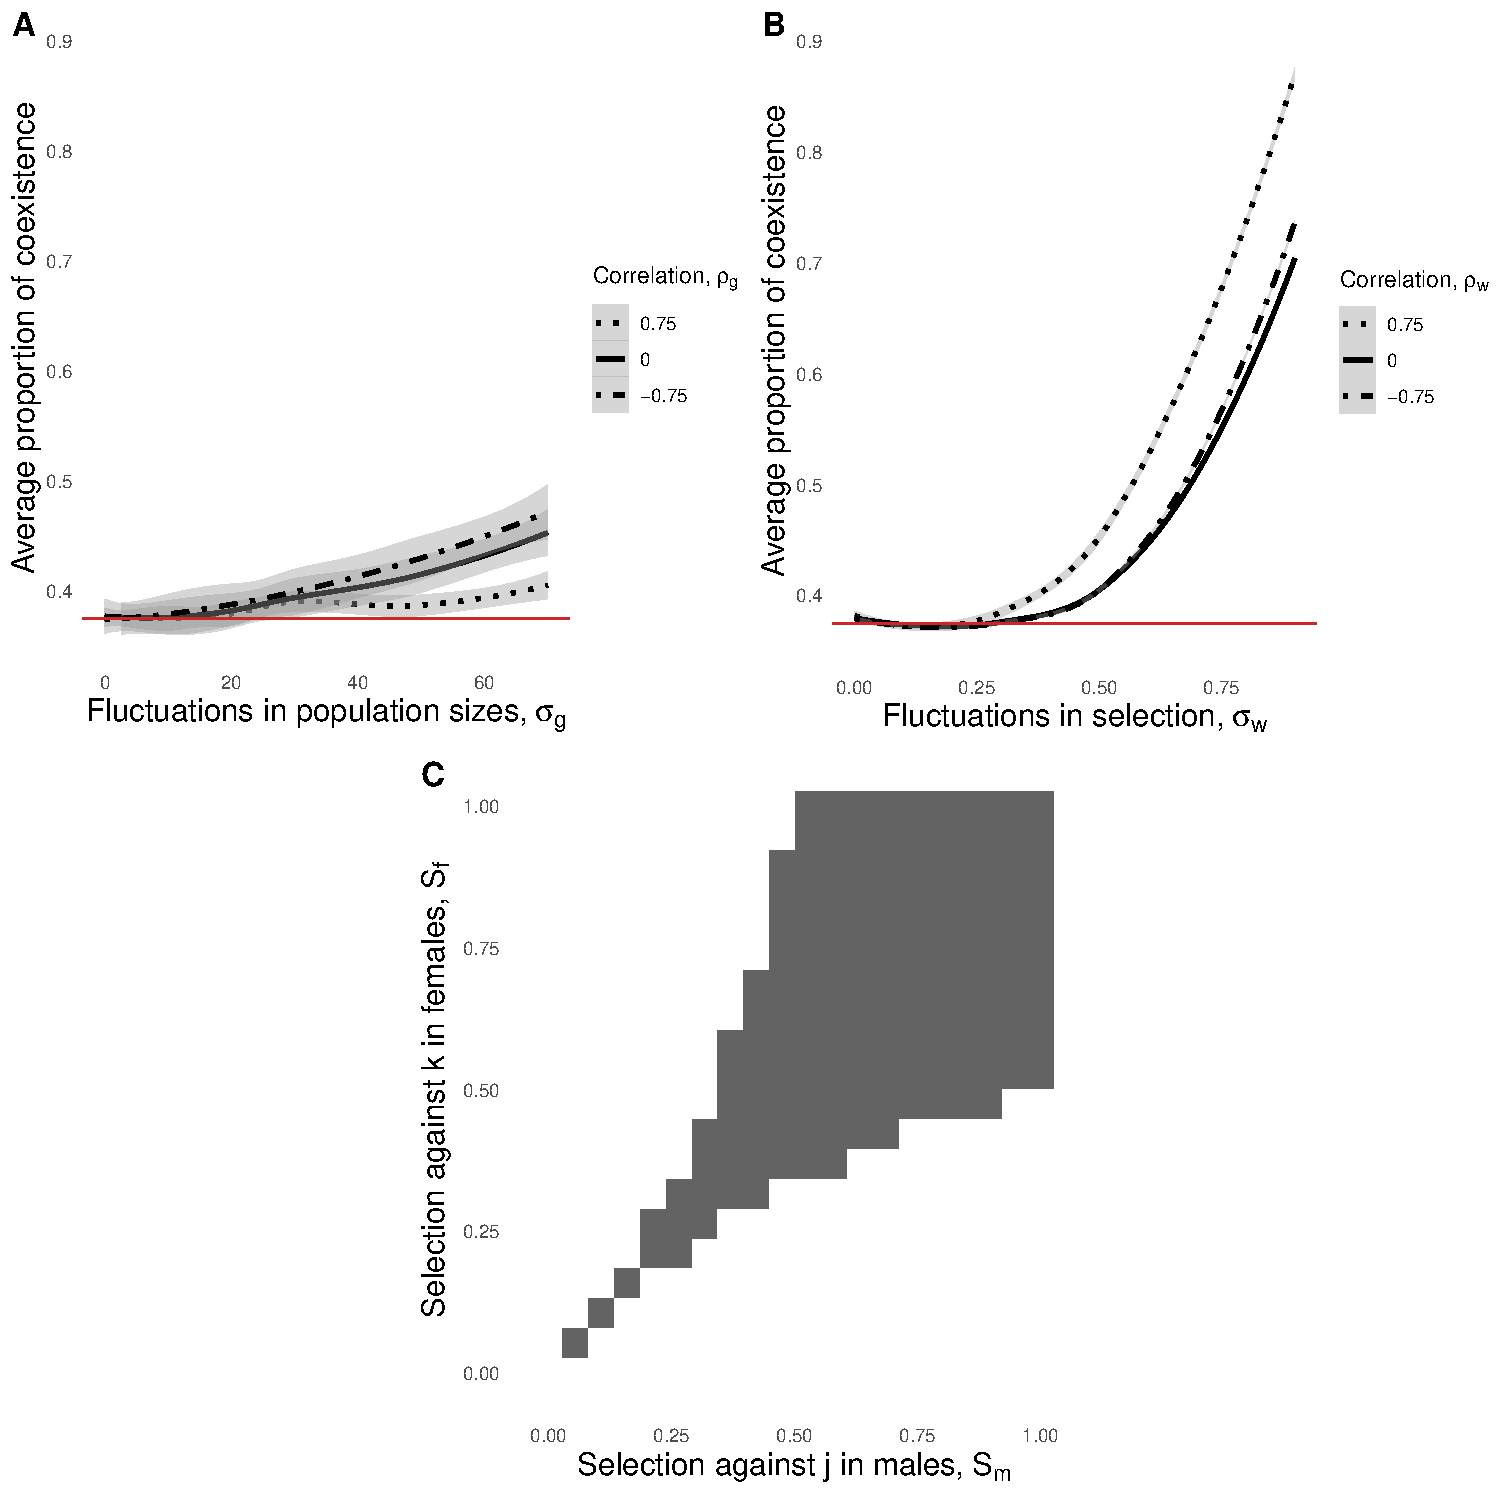
\includegraphics[width=1\textwidth]{proportions.pdf}}
  \caption{}
    \label{fig:prop}
\end{figure}


\clearpage

\begin{figure}[H]
  \centerline{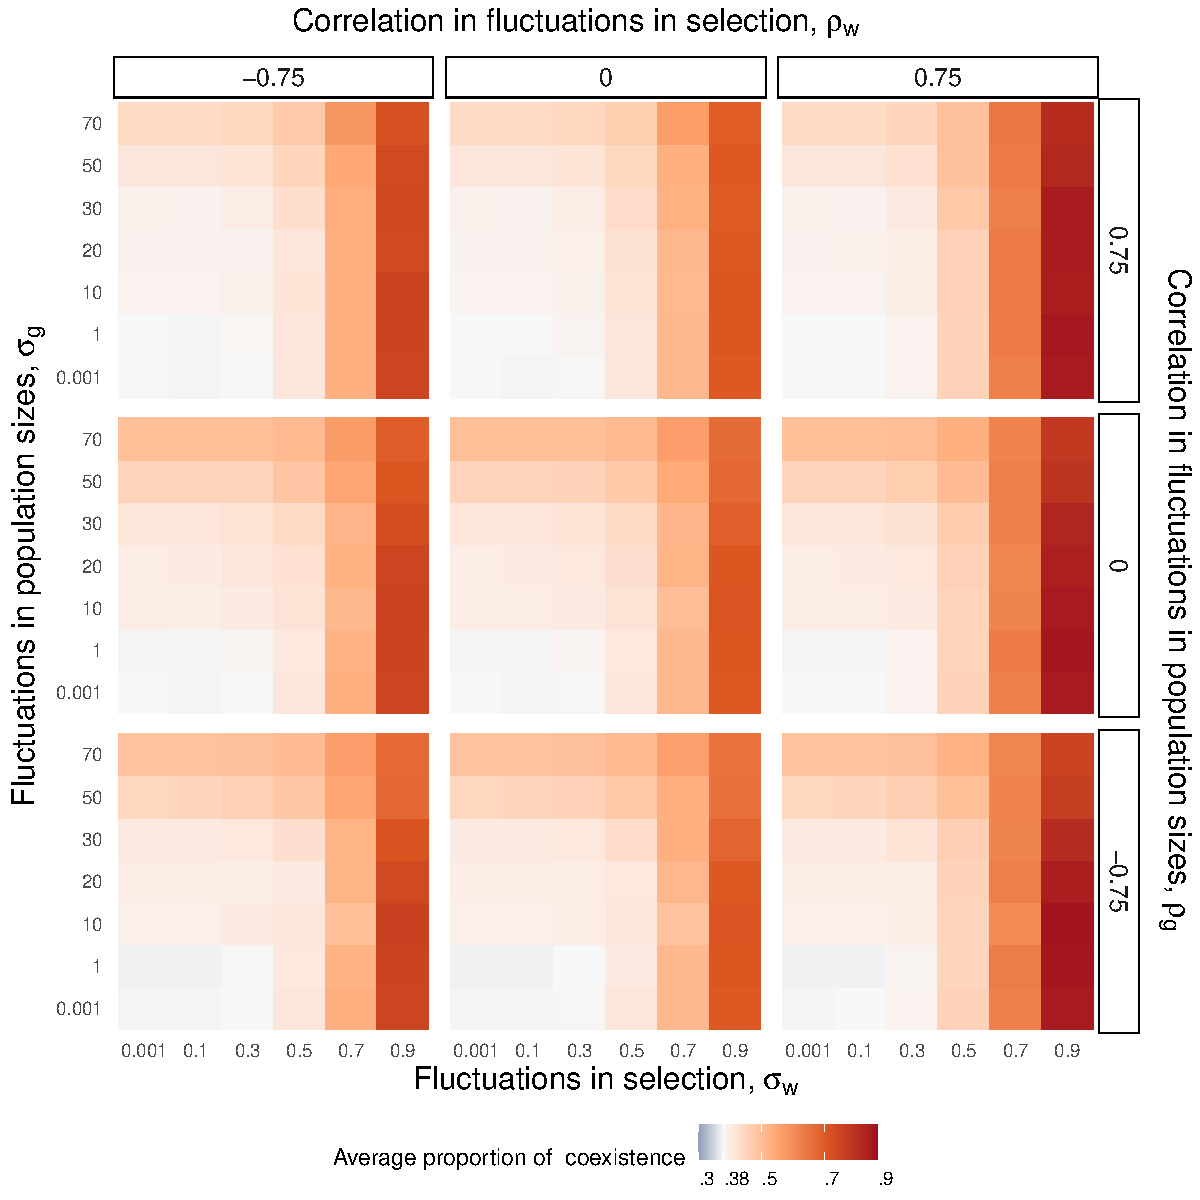
\includegraphics[width=1\textwidth]{heat_map.pdf}}
  \caption{}
    \label{fig:heat}
\end{figure}


\clearpage

\begin{figure}[H]
  \centerline{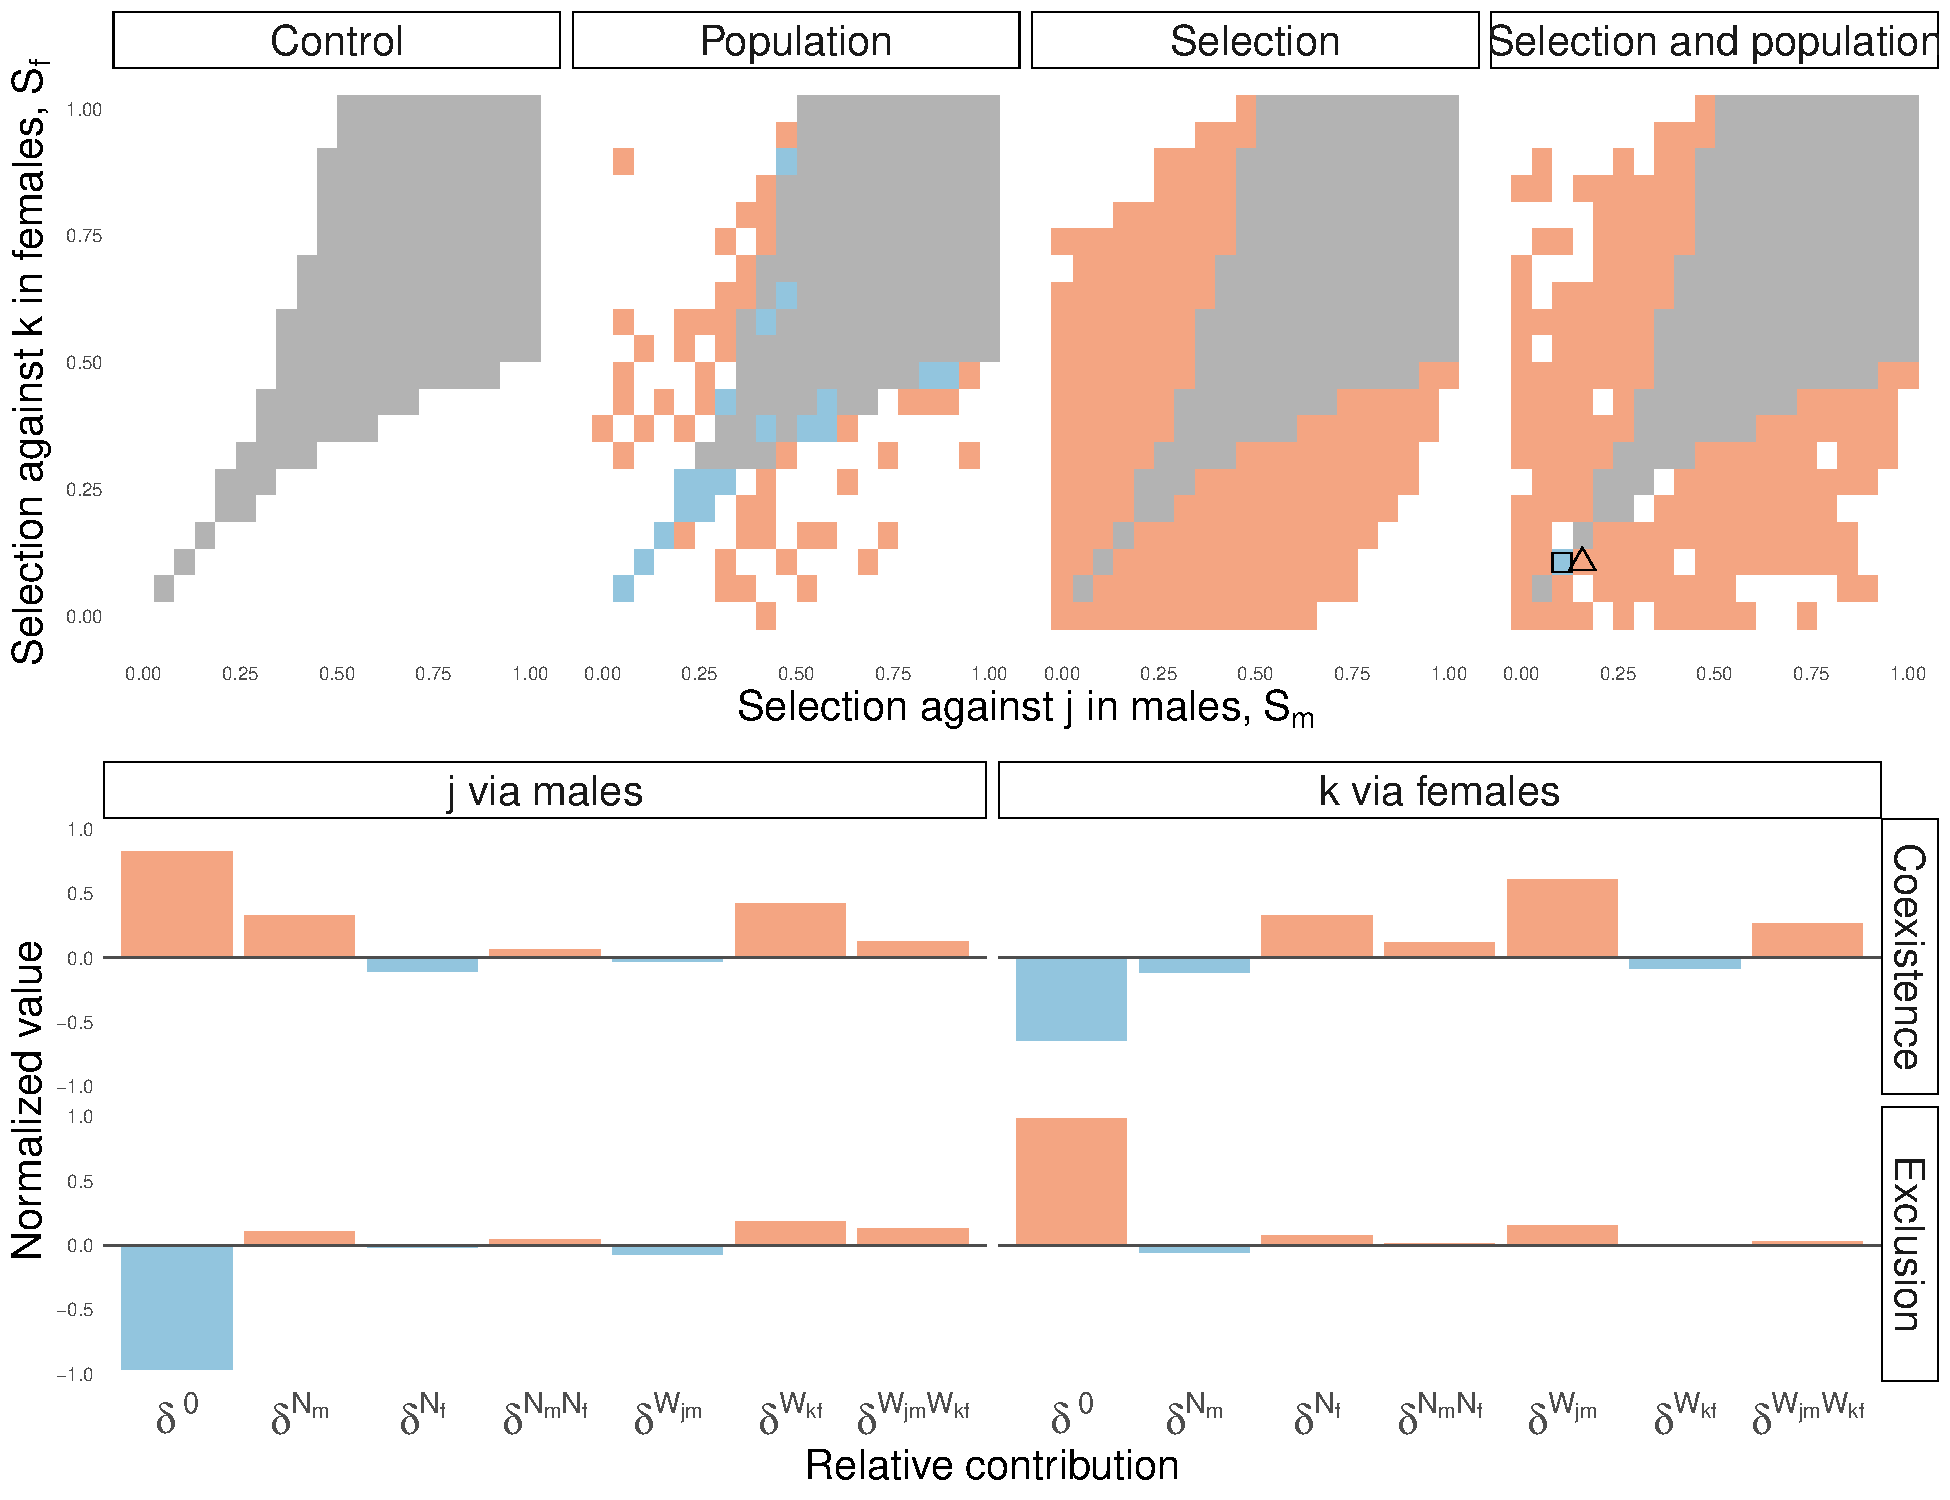
\includegraphics[width=1\textwidth]{outcomes.pdf}}
  \caption{}
    \label{fig:outcomes}
\end{figure}




\begin{figure}[H]
  \centerline{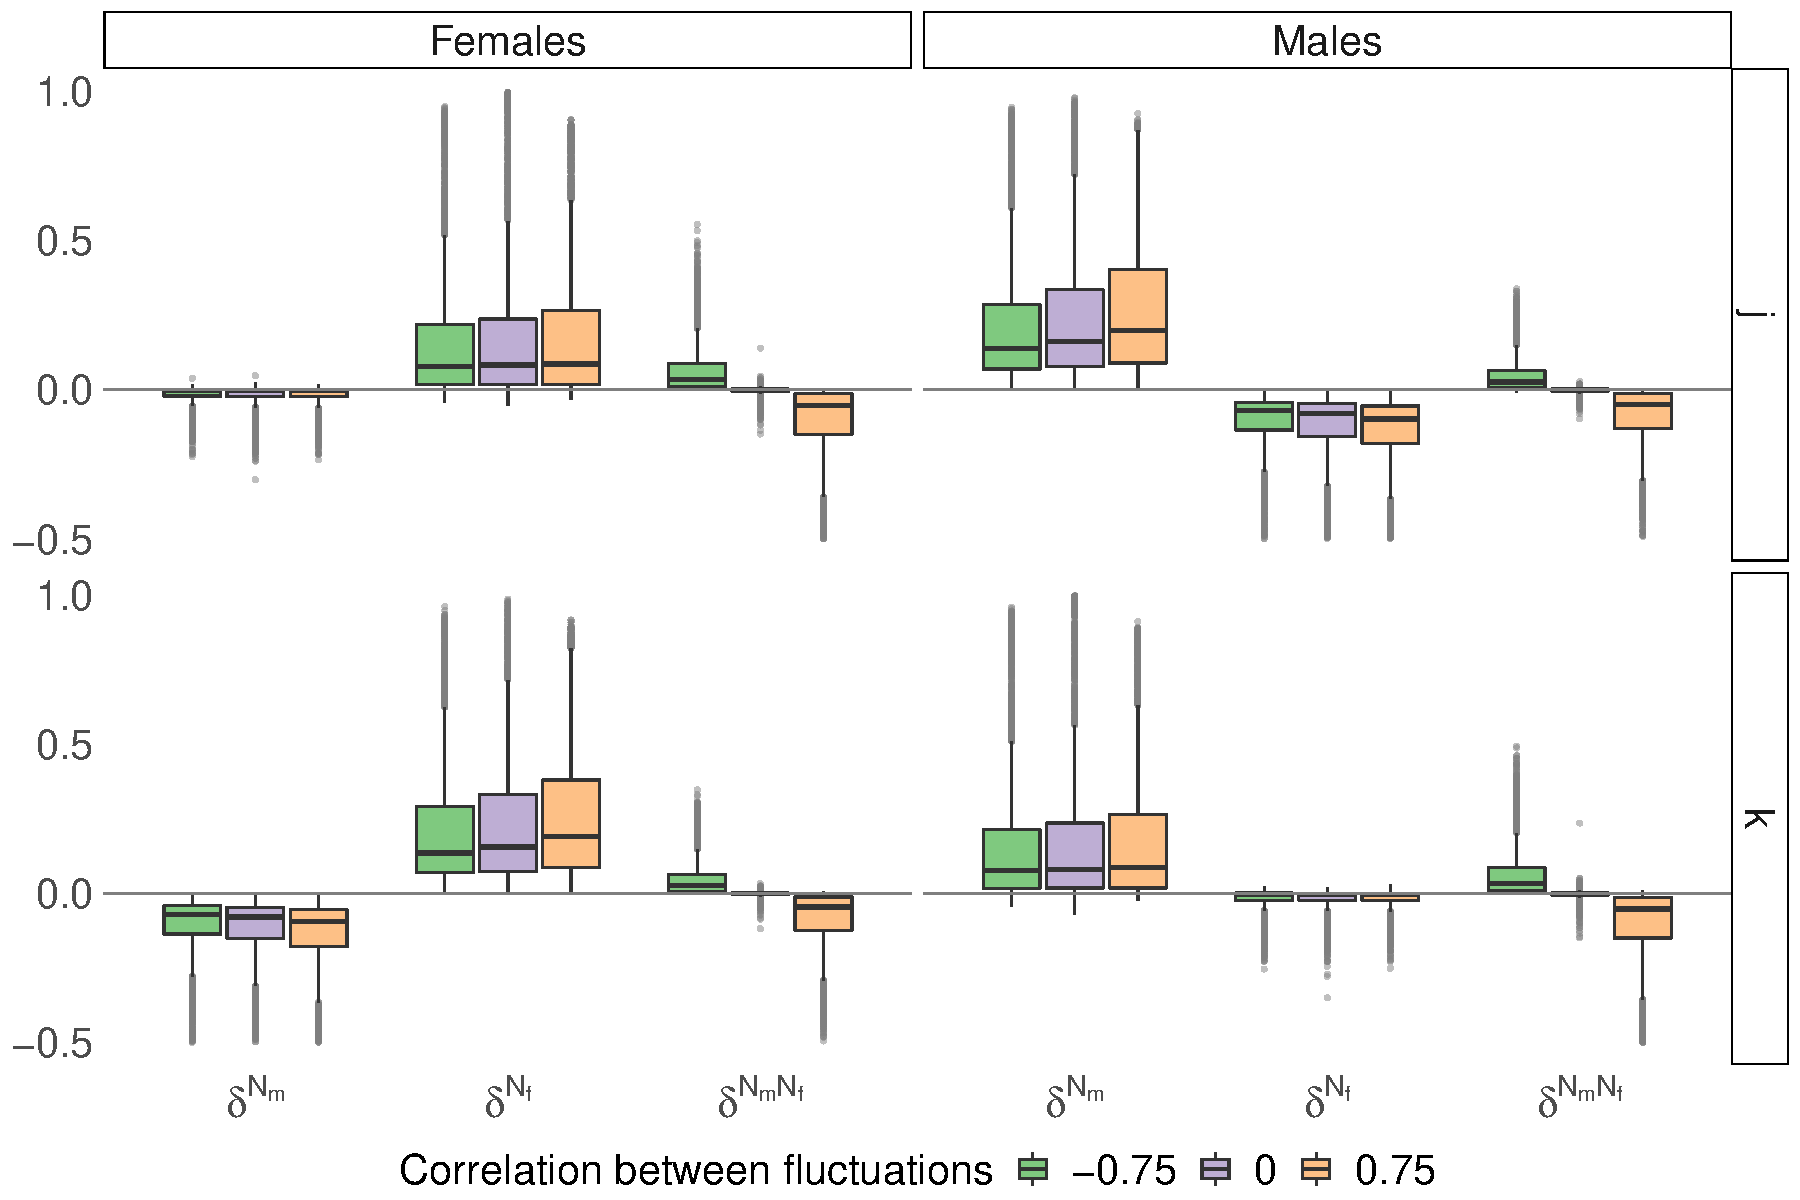
\includegraphics[width=1\textwidth]{box_plots.pdf}}
  \caption{}
    \label{fig:outcomes}
\end{figure}


%\begin{figure}[h]
%  \centerline{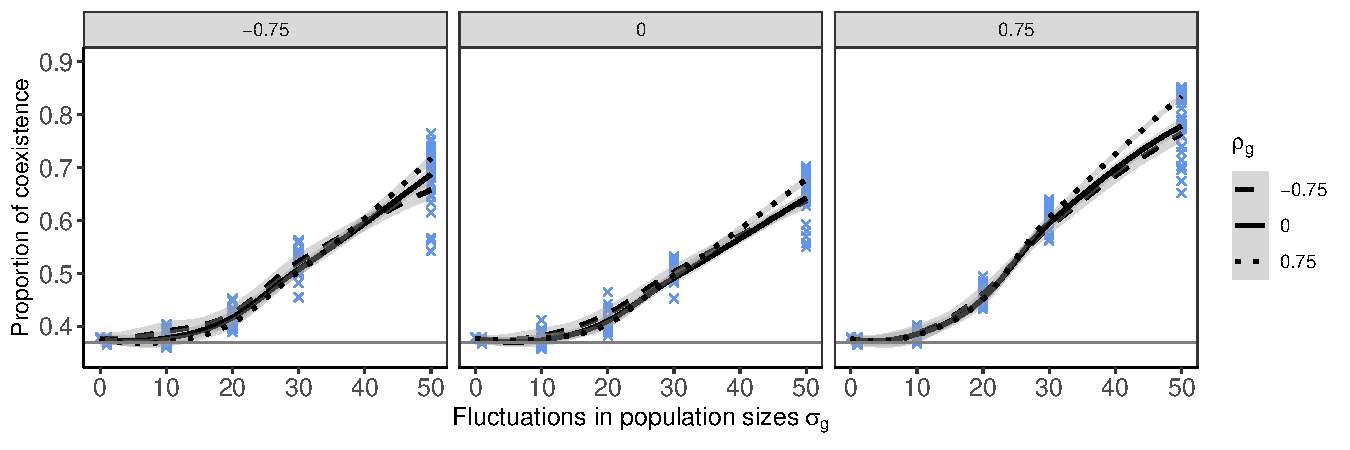
\includegraphics[width=1\textwidth]{fluctuations_two.pdf}}
%  \caption{ }
%    \label{fig:fitness_deltas}
%\end{figure}



\clearpage
\bibliographystyle{ecology_letters}
\bibliography{coexistence.bib}

\end{document}
